\documentclass[a4paper,11pt]{article}
\usepackage[utf8]{inputenc}
\usepackage[T1]{fontenc}
\usepackage[british]{babel}

\usepackage[nodayofweek,level]{datetime}

\usepackage{palatino}

\usepackage{graphicx,xcolor}
\usepackage{hyperref}

\usepackage{csvsimple}



\newcounter{exercisectr}
\setcounter{exercisectr}{0}

\newcommand{\exercise}[1]{%
\par%
\stepcounter{exercisectr}%
\vspace{\baselineskip}%
\noindent\textbf{Exercise \arabic{exercisectr}\ifthenelse{\equal{#1}{}}{}{ : #1}%
.}\quad%
}
\newcommand{\datedownloaded}{\formatdate{05}{11}{2019}}


\begin{document}

\author{Philipp G.~Haselwarter}
\title{Compiling \LaTeX{} with \texttt{make} \\[.2\baselineskip]
  \large Ra\v{c}unalni\v{s}ki praktikum}

\maketitle{}

\begin{abstract}
This is an example of a more complex \LaTeX{} document. The complexity arises because other programs need to be executed before the pdf can be produced from the tex file. Furthermore, every time there is a change made to the files that are included in the tex file (as images, as data table), the pdf report should be reproduced.
\end{abstract}

\section*{Overview}

We download a list of the 50 most popular musical artists from \cite{lastfm}, extract the ten artists with the highest total playcount, produce the plot~\autoref{fig:playcount} from this data, and format the data as table in \autoref{sec:data-table}. To automate this process, we will use the \texttt{make} program~\cite{gnumake}. Furthermore, we give credit to the source of our data and the software we use in the bibliography. As we have seen, this in itself already makes the \LaTeX{} compilation process more complicated.

\begin{figure}[ht]
  \caption{Most popular artists from the \href{https://last.fm/}{last.fm} API \cite{lastfm:API}. Retrived: \datedownloaded{}}
  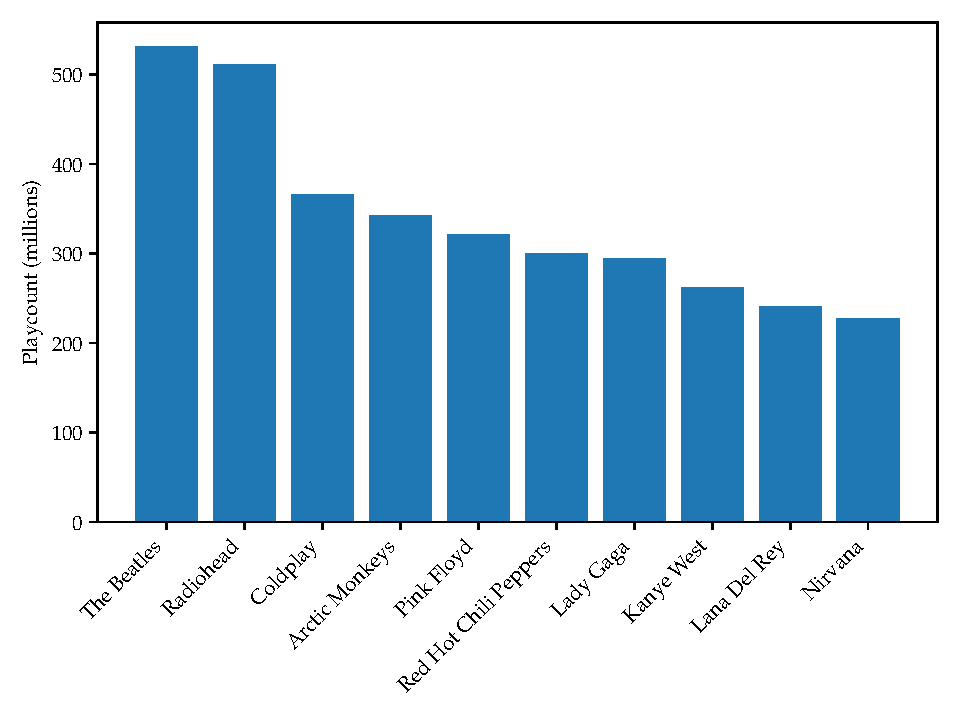
\includegraphics[width=\textwidth]{playcount}
\end{figure}


\tableofcontents{}

\section{Files required to produce this document}

\begin{itemize}
\item \texttt{buildsystem.tex} contains the overall structure and most of the \LaTeX{} code
\item \texttt{literature.bib} contains the literature references we cite
\item \texttt{playcount.pdf} contains a barplot of the play counts of different artists
\item \texttt{top\_artists.csv} contains the data the plot was drawn from
\item \texttt{date\_downloaded.tex} defines a macro that expands to the date when the data was downloaded
\end{itemize}

\section{Steps to produce this document}
\label{sec:steps}

The steps required to compile this document are as follows:
\begin{enumerate}
\item run \texttt{./download\_charts.sh} to produce \texttt{top\_artists.json} and \texttt{date\_downloaded.tex}
\item \label{step:plot} run \texttt{./parse\_charts.py playcount.pdf} to produce \texttt{playcount.pdf}
\item \label{step:csv} run \texttt{./parse\_charts.py top\_artists.csv} to produce \texttt{top\_artists.csv}
\item run \texttt{pdflatex buildsystem.tex} to produce \texttt{buildsystem.aux}
\item run \texttt{bibtex buildsystem} to produce \texttt{buildsystem.bbl}
\item run \texttt{pdflatex buildsystem.tex} twice to fix unresolved references and produce \texttt{buildsystem.pdf}
\end{enumerate}

Observe that steps~\ref{step:plot} and~\ref{step:csv} are independent from each other and can be run in any order.

\exercise{} Open a cygwin terminal, \verb|cd| into your praktikum folder for today, and run these steps to produce \verb|buildsystem.pdf|.

\exercise{} Open \verb|buildsystem.tex| and fix all the tasks masked with \texttt{TODO}.

\exercise{} On a sheet of paper, draw the graph of dependencies between the files. Each node in your graph should correspond to a file, and it should have edges connecting to the files it depends upon. Start with \texttt{buildsystem.pdf}. Does any file depend upon itself? What is a sufficient condition for us to be able to compile a dependency graph? How could we relax that condition?

\section[A simple makefile]{Automating document creation: a simple \texttt{makefile}}

To make compilation more manageable, we would like to leave the steps outlined in~\autoref{sec:steps} to a program instead of performing them manually. Furthermore, and this is important, we want to perform only the steps that are necessary. For example, if we already downloaded the charts, we should not re-perform the download request unless we really want to. Too much stress on the server might result in getting us blocked. The operation would also unnecessarily fail if we already have the data but we're offline. If a node has two or more incoming edges, compilation should still be performed just once.

\subsection{The make program}
\label{sec:make-program}

The \texttt{make} program takes a textual description of the dependency graph together with a \emph{rule} to produce each node from its dependencies or \emph{prerequisites}, and executes the rules to compile the \emph{target}. This description of a compilation process is very general, and can be applied to languages other than latex. The \texttt{make} utility is freely available and runs on all operating systems.

To get an overview of the arguments that \texttt{make} can be invoked with, run \verb|make --help|. The arguments we will be using today are listed in~\autoref{tbl:makeargs}.
%
\begin{figure}[h]
  \centering
  \begin{tabular}[h]{l l l}
    argument & short form & description \\ \hline
    \verb|--help| & \verb|-h| & describe options \& arguments \\
    \verb|--makefile FILE| & \verb|-f FILE| & read rules from \emph{FILE} \\
    \verb|--no-builtin-rules| & \verb|-r| & only use rules from current Makefile \\
    \verb|--debug| & \verb|-d| & explain rule selection during compilation \\
    \verb|--just-print| & \verb|-n| & only print selected rules, no  execution \\
    \verb|--jobs N| & \verb|-j N| & run up to $N$ independent rules in parallel
  \end{tabular}
  \caption{\texttt{make} commandline arguments}
  \label{tbl:makeargs}
\end{figure}
%

\exercise{} Create an empty file called \verb|01-simple.mk| and run
\begin{verbatim}
make -f 01-simple.mk -r -d -n
\end{verbatim}


\subsection{Syntax of Makefiles}
\label{sec:syntax-makefiles}

Text editors recognise files with the extension \verb|.mk| as makefiles. The
syntax for rules is as follows:
%
\begin{verbatim}
target : prerequisite-1 prerequisite-2 [...]
\tab  recipe
\end{verbatim}
%
where \verb|\tab| should be an actual tab character, not followed by spaces. \verb|target| and the list of \verb|prerequisite-N| are file names. \verb|recipe| is a shell command that should produce \verb|target|, assuming that all prerequisites have been taken care of. For example, to express that \verb|top_artists.csv| depends on \verb|parse_charts.py| and \verb|top_artists.json|, one would write the following rule:
\begin{verbatim}
top_artists.csv : parse_charts.py top_artists.json
\tab	./parse_charts.py top_artists.csv
\end{verbatim}
%
If a target requires the execution of several commands, the commands should be listed under the target, each indented with a tab, one command per line.
%
Comments can be started with a \verb|#| character. Long lines may be broken by putting a \verb|\| at the end of the line and continuing on the next line.


\exercise{} Add a rule for each node in the dependency graph to \verb|01-simple.mk|. Start with those nodes that are leafs in the graph, i.e. that do not depend on any further files. While you add rules, run \verb|make| with the correct arguments to see what actions would get performed. You can specify the target you want to build by adding it as a last argument to the make invocation. By default, the first target listed in the makefile will be selected. Once you're done, delete all the intermediate files with
%
\begin{verbatim}
  rm *.pdf *.log *.blg *.bbl *.aux
\end{verbatim}
%
and build the pdf again.

\exercise{} Add two more rules to \verb|01-simple.mk|: \verb|clean| should delete all files ending in \verb|.log .aux .blg .bbl|, \verb|extraclean| should run \verb|clean| and additionally delete the following files:
\begin{itemize}
  \setlength{\itemsep}{0pt}
\item \verb|buildsystem.pdf|
\item \verb|top_artists.json|
\item \verb|date_downloaded.tex|
\item \verb|playcount.pdf|
\item \verb|top_artists.csv|
\end{itemize}

\section{Writing a sophisticated \texttt{makefile}}

Now that we have a basic \texttt{makefile} working, let's explore some more features of \texttt{make}. Create a new file \verb|02-fancy.mk| based on \verb|01-simple.mk|.

\exercise{phony targets} The last two rules that we added, \verb|clean| and \verb|extraclean|, do not actually create any files. However, if through some other means a file called \verb|clean| was actually put into the folder, the \texttt{make} would not execute the \verb|clean| rule anymore. In \texttt{make} terminology, such rules are \emph{phony}. Here is the Witionary entry for \emph{phony (noun)}:
%
\begin{quote}
  A person who assumes an identity or quality other than their own. \\
  Example: ``He claims to be a doctor, but he's nothing but a fast-talking phony.''
\end{quote}
%
We can declare a targets as phony by listing them as prerequisites for a special \texttt{make} target called \verb|.PHONY|.

\exercise{failing} Make sure that the file \verb|buildsystem.pdf| exists. Run \texttt{make} on the \verb|clean| target. Then run \verb|extraclean|. The file \verb|buildsystem.pdf| did not get deleted. Why did \texttt{make} fail? Read the manual for the \texttt{rm} command by running \verb|man rm| (use \texttt{page up/down} to navigate, press \texttt{q} to quit), and find an option that modifies the behaviour of \texttt{rm} so that \verb|clean| does not fail in this situation.

\exercise{multiple targets} The files \verb|top_artists.json| and \verb|date_downloaded.tex| are produced by identical rules. In fact, a rule can have more than one target. List the targets in a single rule. Targets are simply separated by a space, like prerequisites.

\exercise{defining variables} The file names \verb|playcount.pdf| and \verb|top_artists.csv| occur together several times in the makefile. We can define a variable as follows:
\begin{verbatim}
SCRIPT_TARGETS = playcount.pdf top_artists.csv
\end{verbatim}
%
and then reference it as \verb|$(SCRIPT_TARGETS)|. Replace occurances of the two file names by the variable. Then repeat the process for a variable \verb|DOWNLOAD_TARGETS| for the files that \verb|download_charts.sh| produces.

\exercise{built-in variables} The files in \verb|$(DOWNLOAD_TARGETS)| are created by the exact same command. The situation is very similar for \verb|$(SCRIPT_TARGETS|, except that in each case the argument to \verb|./parse_charts.py| has to be replaced by the name of the target. We can access the name of the current target when a recipe is executed under the variable \verb|$@|. Modify the rules for \verb|playcount.pdf| and \verb|top_artists.csv| so that the recipe does not explicitly mention the name of the target anymore but uses \verb|$@| instead. Then combine the two rules into a multi-target rule.

\exercise{more variables} It is good practise to define a variable for the name of the program that compiles the main target, in our case \verb|pdflatex|, and a variable for the arguments to that program. This way, if the arguments change, they can be conveniently edited at the beginning of the file. Define a compiler variable for \verb|pdflatex| and set the argument variable to \verb|-synctex=1|. Then use these variables in the rest of the makefile instead.

\section{Modern problems need modern solutions}

The \texttt{make} utility is a very useful general purpose tool. However, \LaTeX{} has some peculiarities that require special solutions. In particular, after \verb|bibtex| is run, we have to invoke \verb|pdflatex| twice more. In fact, there are some scenarios where even a third invocation is required. This makes it difficult to write robust makefiles. A solution would be to parse the log files and check whether \verb|pdflatex| or some other package requires another pass. The \verb|latexmk| utility does exactly that. For simple projects that require no external programs to be run besides \verb|bibtex|, it can completely replace a makefile.

Create a new file \verb|03-latexmk.mk| based on \verb|02-fancy.mk|.

\exercise{} Replace the two consecutive invocations of \verb|pdflatex| in the rule for \verb|buildsystem.pdf| by a single call to \verb|latexmk|. Be sure to add the \verb|-pdf| option to the variable that defines the arguments for the \LaTeX{} compiler. As \verb|latexmk| how to produce a \verb|.aux| file, the rule for \verb|buildsystem.aux| will now be obsolete.

\exercise{} What does \verb|latexmk -c| do? What does \verb|latexmk -C| do? Modify your new makefile to use this functionality.

\section{Exploring the \texttt{last.fm} API}
\label{sec:lastfm-api}

\exercise{bonus} Read the documentation of the \texttt{last.fm} application programming interface~\cite{lastfm:API}. The \verb|download_charts.sh| script uses the \texttt{chart.getTopArtists} method of the API. Create a script \verb|download_top_tracks.sh| that uses \texttt{chart.getTopTracks} method instead, and save the result to \verb|top_tracks.json|.

\exercise{bonus} Modify \verb|parse_charts.py| so that it can also parse the top tracks and output a plot like the one for artists, as well as a corresponding csv file.


\bibliographystyle{apalike}
\bibliography{literature}

\appendix

\section{Data table}
\label{sec:data-table}

\csvautotabular{top_artists.csv}
% TODO : use the \csvautotabular command to include the table from top_artists.csv


\end{document}
